\documentclass[9pt, english, a4paper]{article}
\usepackage[latin1]{inputenc}
\usepackage[T1]{fontenc}
\usepackage{babel,graphicx, mathpple, textcomp, varioref, listings, color, colortbl, amssymb, amsthm}
\input{kvmacros}


\bibliographystyle{plain} % or: "chicago"
%\usepackage{natbib} % a citation management package

\usepackage[sort&compress]{natbib}

\theoremstyle{definition}
\newtheorem{definition}{Definition}[section]

\title{The path to true concurrency\\(Sculptures, ST-structures and HDAs)}
\author{Christopher A. Trotter \\ Department for informatics\\ University of Oslo}

\date{\today{}}

\tolerance = 10000 		% LaTeX er normalt streng når det gjelder linjebrytingen.
\hbadness = \tolerance 	% Vi vil være litt mildere, særlig fordi norsk har så
\pretolerance = 2000	% mange lange samensatte ord.

\begin{document}

\maketitle{}

\begin{abstract}
	\noindent The main purpose is to provide concrete relationships between highly expressive concurrency models coming from two different schools of thought: the higher dimensional automata, a state-based approach by Pratt and van Glabbeek; and the configuration structures and unrestricted event structures, an event-based approach by van Glabbeek and Plotkin. In this respect, we will define the method of sculpting, described by Pratt, in categorical terms to better understand the event-state duality defined by Pratt. These investigations of sculptures in category theory are intended to provide a better understanding of the relationship between ST-structures, HDAs and Sculptures in terms of expresiveness. 
	%Moreover, we intend to provide an example of a HDA which can not be sculpted by the categorical definition of a sculpture. 
	%\noindent We will provide a formal description of sculpting which is similar to what Pratt has used in [x] wrt. higher dimensional automata(HDA) and ST-structures(ST). For this task we must deal with the expressiveness and correspondance of the above models. In particular the relationship between the HDAs and sculptures.
\end{abstract}



\section{Introduction}
	%In highly expressive concurrency models, HDA is a state-based approach by Pratt and van Glabeek and is a geometric model of concurrency that has an attractive aspect which is the automata-like presentation. This aspect is opposed to the event-based models of concurrency, like (prime, flow, (non-)stable) event structures [x, y, z] or configuration structures such as ST.\\

	%One of the most commonly used models of concurrency is that of automata, also known as process graphs, state transition diagrams or labelled transition systems. In ordinary automata, the parallel composition of two actions a and b is displayed as a process P that executes a and b in either order, ending in the same state each way, such that a and b are mutually exclusive. Throughout the years, people have wondered whether the elegance of automata could be combined with the expresiveness of models like (prime, flow, (non-)stable) event structures[5, 6, 7] or configuration structures and unrestricted event structures[8, 9]. The geometric model of concurrency, studied by Pratt and van Glabbeek [1, 2, 3], is of high expressive power, thus providing a general framework for studying the difference and common features of various other models of concurrency(as done in [3] and [4]). This model was named Higher Dimensional Automata(HDA) by Pratt[1]. An attractive aspect of HDA is the automata-like presentation[3], which emphasizes the state aspect of the modelled system(and transitions between states). The idea of HDA had to some extent been contempllated before in [28] and applied in [23]. However, [24] offered the first formalisation of the idea and Pratt's formalisation was based on n-categories.

	%Throughout the years, people have wondered whether the elegance of automata could be combined with the expressiveness of models like (prime, flow, (non-)stable) event structures[5, 6, 7] or configuration structures and unrestricted event structures[8, 9]. 



	%One of the most commonly used models of concurrency is that of automata, also known as process graphs, state transition diagram or labelled transition systems. In ordinary automata, the parallel composition P of two actions a and b is displayed in the same way as a system M that executes a and  b in either order, ending in the same state each way, such that a and b are mutually exclusive.

	One of the most commonly used models of concurrency is that of automata, also known as process graphs, state transition diagrams or labelled transition systems. In ordinary automata, the parallel composition of two actions \emph{a} and \emph{b} is displayed as a process \emph{P} that executes \emph{a} and \emph{b} in either order, ending in the same state each way, such that \emph{a} and \emph{b} are mutually exclusive. There is a hidden assumption of excluded middle as described by Pratt in \cite{pratt1991}, such that the dual of a true concurrency schedule appears to be a false concurrency automaton.

	This has lead to the geometric model of concurrency, studied by Pratt and van Glabbeek \cite{pratt1991, pratt2000, glab2006}, which is of high expressive power, thus providing a general framework for studying the difference and common features of various other models of concurrency(as done in \cite{glab2006} and \cite{goub2012}). This model was named Higher Dimensional Automata(HDA) by Pratt\cite{pratt1991}. HDAs retained the state-based view and models $a||b$ as the evident four-state $"$square$"$ automaton accepting ab + ba, but with its square interior filled in(Section 2). This aspect is opposed to the event-based model of concurrency, like (prime, flow, (non-)stable) event structures\cite{winsk1979, winsk1986,castell1989} or configuration structures and unrestricted event structures\cite{glab1995, glab2009}.

	%This lead to
	%In response to the ordinary automata, both event-based and geometry-based approaches to concurrency were developed. Event structures replace the traditional state-based view of computation by the view of $a||b$ as a set $\{a,b\}$ representing two events unconstrained as to order. In contrast the geometry-based approach retains the state-based view and models $a||b$ as the evident four-state $"$square$"$ automaton accepting ab + ba but with its square interior filled in.

	%This lead to the geometric model of concurrency, studied by Pratt and van Glabbeek [1, 2, 3], which is of high expressive power, thus providing a general framework for studying the difference and common features of various other models of concurrency(as done in [3] and [4]). This model was named Higher Dimensional Automata(HDA) by Pratt[1]. An attractive aspect of HDA is the automata-like presentation[3], which emphasizes the state aspect of the modelled system(and transitions between states). This aspect is opposed to the event-based model of concurrency, like (prime, flow, (non-)stable) event structures[5, 6, 7] or configuration structures and unrestricted event structures[8, 9].

	We are interested in studying such models based on sets of event, but in relation to the state-based model of higher dimensional automata. This study of event-state duality is argued by Pratt\cite{pratt2002}, and the model of chu spaces has been developed in response[13, 14].

	Here the challenge of Pratt with insight from chu spaces and the models based on sets of event, in the spirit of van Glabbeek and Plotkin\cite{glab2009}, are addressed in [ST-paper](Section 3). This model was named ST-structures(ST)[ST-paper]. The relationship between ST-structures and HDAs gives an intuition of the event-state duality described by Pratt, and the method of sculpting gives the relation between ST-structures and HDAs.

	%The geometric model of concurrency, studied by Pratt and van Glabbeek [1, 2, 3], is of high expressive power, thus providing a genereal framework for studying the difference and common features of various other models of concurrency(as done in [3] and [4]). This model was named Higher Dimensional Automata(HDA) by Pratt[1]. An attractive aspect of HDA is the automata-like presentation[3], which emphasizes the state aspect of the modelled system(and transitions between states). This aspect is opposed to the event-based models of concurrency, like (prime, flow, (non-)stable) event structures[5, 6, 7] or configuration structures and unrestricted event structures[8, 9].

	%We are interested in studying such models based on sets of events, but in relation to the state-based model of higher dimensional automata. This study of event-state duality is argued by Pratt[12], and the model of chu spaces has been developed in response[13, 14]. Here the challenge of Pratt, with insight from chu spaces and the developed models based on sets of event, in the spirit of van Glabeek and Plotking[9] have been named ST-structures(ST) in [ST-paper]. The relationship between ST and HDA give an intuition of the event-state duality described by Pratt. In this respect, we provide a formal definition of the method of sculpting which is much like what Pratt has used in [?, 2] to better describe the event-state duality. 


	%The main purpose of this paper is to provide a formal definition of Pratt's notion of sculptures in categorical terms. In this regard, highly expressive concurrency models such as ST-structures(ST) and higher dimensional automata(HDA) have show to have strong relations to the notion of sculptures. In the state-event duality both ST and HDA 

	%- We give a formal method to describe the notion of sculpting based on category theory.
	%- We prove that the HDA example figure can not be sculpted by definition of the formal method.
	%- We provide by the example a counter argument to the notion of sculpting and define a refined notion of sculpting.

	%Note: Start with an example that illustrates the problem. (figure 6 left)

	%1. Describe the problem(the lack of a formal definition of sculpting)\\
	%	- Here is a problem\\
	%	- Its an interesting problem because ...\\
	%	- Its an unsolved problem\\
	%	- here is my claim to solving the problem\\


	%2. State your contribution(A formal method to defining what sculpting is in category theory)\\
	%	- We provide an understanding of the relationships between HDA and ST-structures, ST-structures and sculptures and especially HDA and sculptures.\\
	%	- We give a formal method to describe the notion of sculpting based on category theory.
	%	- We prove that the HDA example figure can not be sculpted by definition of the formal method.
	%	- We provide by the example a counter argument to the notion of sculpting and define a refined notion of sculpting.

	%Note: Start with an example that illustrates the problem. (figure 6 left)

	%Introduce what this concept of sculpting is.
	%Say something about its connection to HDA and ST based on the paper on ST-structures.

	%In highly expressive concurrency models, higher dimensional automata, known as HDA, is a state-based approach by Pratt and van Glabeek. HDA is a geometric model of concurrency that has an attractive aspect which is the automata-like presentation. On the other hand, from a different school of thought there are configuration structures and unrestricted event structures which is a event-based approach by van Glabeek and Plotkin. For the event-based approach, the model of ST-structures which is a configuration structure investigated in [Q] is intended to provide a better understanding of the state-event duality described by Pratt. In this respect we will investigate and formulate the method of sculpting, which is similar to what Pratt has used in [w]. Moreover, we have preliminary results from a categorical approach of the relationship between HDA and sculpting.
	
	%The main purpose is to investigate and formulate sculpting which is similar to what Pratt has used in [z]  wrt. two different school of thought: the higher dimensional automata, a state-based approach by Pratt and van Glabeek; and the configuration structures and unrestricted event structures, an event-based approach by van Glabeek and Plotkin. For the event-based approach, we will investigate ST-structures in [x] to provide a better understanding of the state-event duality described by Pratt. Moreover, we will study the relationships between ST-structures and sculptures, HDA and sculptures and ST-structures and HDA. Especially the relationship between HDA and sculptures based on the notion Pratt provides in [y]. As for providing a more formal description, we have preliminary results from a categorical approach describing the relation of sculptures to HDAs.\\

\section{HDA}
	
	\theoremstyle{definition}
	\begin{definition}{\textbf{(higher dimensional automata [3, Def.1])}}\\
		\indent A cubical set H = (Q, $\bar{s}$, $\bar{t}$) is formed of a family of sets Q=$\cup_{n=0}^{\infty}$ $Q_{n}$ with all sets $Q_{n}$ disjoint, and for each n, a family of maps $s_{i}$, $t_{i}$ : $Q_{n} \rightarrow Q_{n-1}$, with $1 \leq i \leq i \leq n$, which respects the following cubical laws:

		\begin{equation}
		\alpha_{i} \circ \beta_{j} = \beta_{j-1} \circ \alpha_{i},\ 1 \leq i < j \leq n\ and\ \alpha, \beta \in \{s,t\}.
		\end{equation}

		\noindent In H, the $\bar{s}$ and $\bar{t}$ denote the collection of all the maps from all the families (i.e., for all n).A higher dimensional automaton (Q, $\bar{s}$, $\bar{t}$, l, F) over an alphabet $\sigma$ is a cubical set together with a labelling function l:$Q_{1} \rightarrow \sigma$ which respects $l(s_{i}(q))$ = $l(t_{i}(q))$ for all $q \in Q_{2}$ and $i \in \{1,2\}$; and with $I \in Q_{0}$ initial and $F \subset Q_{0}$ final cells.\\

		The elements of $Q_{0}$ are called nodes and those of $Q_{1}$, $Q_{2}$ and $Q_{3}$ are \emph{edges, square} and \emph{cubes}, respectively. In general, the elements of $Q_{n}$ are called \emph{n-dimensional hypercubes}, or \emph{n-cells}. An n-dimensional hypercube represents a state of a concurrent system in which n transitions are firing concurrently. Because the dimensions of the hypercube are numbered 1,...,n, these transitions are de facto stored as a list.

	\end{definition}



\section{ST-structures}
	We define ST-structures, showing in Section 3 that they are a natural extension of configuration structures[9], and define related notions that stem from the latter. The classical notions of concurrency, causality and conflict are not interdefinable as in the case of event structures or stable configuration structures; but are more loose, as in the case with HDAs.

	\theoremstyle{definition}
	\begin{definition}{\textbf{(ST-structures)}}
		An ST-configuration structure(also called ST-structure) is a tuple ST = (E, ST, l) with ST a set of ST-configurations over E satisfying the constraint:

		\begin{equation}
			if(S,\ T) \in ST\ then\ (S,\ S) \in ST,
		\end{equation}

	\noindent and l:$E \rightarrow \sigma$ a labelling function with $\sigma$ the set of labels. We often omit the set of events E from the notation when  there is no danger of confusion.\\

	The contraint(2) above is a closure, ensuring that we do not represent events that are started but never terminated. he set of all ST-structures is denoted $ST$. 

	\end{definition}


\section{Sculptures}


%prove that HDA is isomorphic to sculptures


\section{event structures / configuration structures}



\section{Results/just future plans}



\subsection{category theory relate sculptures}



\subsubsection{through ST structures}



\subsection{proof of non-sculpture}

	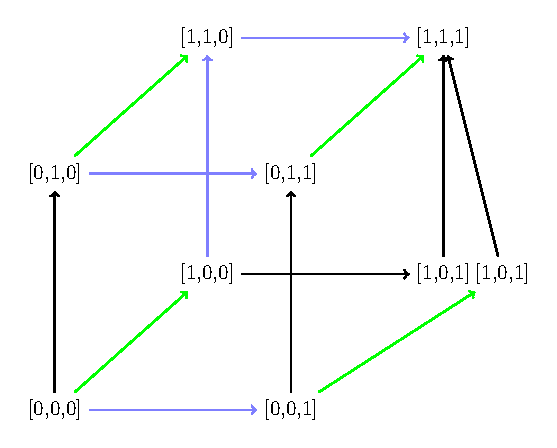
\includegraphics[scale=0.7]{illustrations/figure6.pdf}

	%Pratt gives us the general notion of sculptures, but leaves us without formally defining what this can be. Uli Fahrenberg has given a categorical definition to the high-level abstraction of sculptures and that is given as such.....

	%Having a clear understanding of an abstract notion in itself is a result. This is what should be focused on in the abstraction and be the main motivation for writting the submission to CONCUR. This should be a comparison approach to other formal models... this can be done through comparing Chu Spaces, HDA, ST, Sculptures, etc.

	%We have gotten some preliminary results which are indeed important to determine the concept of a Sculpture and what it means. Also to refine the placement of sculptures meaning that it might be more well behaved than HDAs since there is some information lost in translation between ST and HDA, but ST and Sculptures seem to be equally expressive. So what is the cause of this?

	%NOTE: write out everything that then work on shrinking the ideas and concepts found. This is a good practice to be able to write long and difficult texts as well as getting better at being more concrete and decisive on what is important for the topic.


	%Concurrency theory in theoretical computer science deals with methods, problems and algorithms occurring along with parallel computations. Higher-dimensional Automata are particular models for the study of concurrency; they can be described in a combinatorial/topological manner that takes particular care of the time flow. An analysis of these models has to incorporate direction into tools and methods from algebraic topology and gives rise to \"directed algebraic topology\". The main aim is an analysis of the properties of spaces of executions ( = directed paths) in Higher Dimensional Automata.

	\noindent \textbf{Achnowledgements:} The work on Sculptures was guided by Christian Johansen and Uli Fahrenberg.
	\bibliography{./references/references.bib}


\end{document}